\documentclass[12pt,t]{beamer}
\usepackage{graphicx}
\setbeameroption{hide notes}
\setbeamertemplate{note page}[plain]
\usepackage{listings}

% get rid of junk
\usetheme{default}
\beamertemplatenavigationsymbolsempty
\hypersetup{pdfpagemode=UseNone} % don't show bookmarks on initial view


% font
\usepackage{fontspec}
\setsansfont
  [ ExternalLocation = fonts/ ,
    UprightFont = *-regular ,
    BoldFont = *-bold ,
    ItalicFont = *-italic ,
    BoldItalicFont = *-bolditalic ]{texgyreheros}
\setbeamerfont{note page}{family*=pplx,size=\footnotesize} % Palatino for notes
% "TeX Gyre Heros can be used as a replacement for Helvetica"
% I've placed them in ../fonts/; alternatively you can install them
% permanently on your system as follows:
%     Download http://www.gust.org.pl/projects/e-foundry/tex-gyre/heros/qhv2.004otf.zip
%     In Unix, unzip it into ~/.fonts
%     In Mac, unzip it, double-click the .otf files, and install using "FontBook"

% named colors
\definecolor{offwhite}{RGB}{255,250,240}
\definecolor{gray}{RGB}{155,155,155}

\definecolor{background}{RGB}{255,255,255}
\definecolor{foreground}{RGB}{24,24,24}
\definecolor{title}{RGB}{27,94,134}
\definecolor{subtitle}{RGB}{22,175,124}
\definecolor{hilit}{RGB}{122,0,128}
\definecolor{vhilit}{RGB}{255,0,128}
\definecolor{lolit}{RGB}{95,95,95}

\definecolor{nhilit}{RGB}{128,0,128}  % hilit color in notes
\definecolor{nvhilit}{RGB}{255,0,128} % vhilit for notes

\newcommand{\hilit}{\color{hilit}}
\newcommand{\vhilit}{\color{vhilit}}
\newcommand{\nhilit}{\color{nhilit}}
\newcommand{\nvhilit}{\color{nvhilit}}
\newcommand{\lolit}{\color{lolit}}

% use those colors
\setbeamercolor{titlelike}{fg=title}
\setbeamercolor{subtitle}{fg=subtitle}
\setbeamercolor{institute}{fg=lolit}
\setbeamercolor{normal text}{fg=foreground,bg=background}
\setbeamercolor{item}{fg=foreground} % color of bullets
\setbeamercolor{subitem}{fg=lolit}
\setbeamercolor{itemize/enumerate subbody}{fg=lolit}
\setbeamertemplate{itemize subitem}{{\textendash}}
\setbeamerfont{itemize/enumerate subbody}{size=\footnotesize}
\setbeamerfont{itemize/enumerate subitem}{size=\footnotesize}

% page number
\setbeamertemplate{footline}{%
    \raisebox{5pt}{\makebox[\paperwidth]{\hfill\makebox[20pt]{\lolit
          \scriptsize\insertframenumber}}}\hspace*{5pt}}

% add a bit of space at the top of the notes page
\addtobeamertemplate{note page}{\setlength{\parskip}{12pt}}

% default link color
\hypersetup{colorlinks, urlcolor={hilit}}

\ifx\notescolors\undefined % slides
  % set up listing environment
  \lstset{language=bash,
          basicstyle=\ttfamily\scriptsize,
          frame=single,
          commentstyle=,
          backgroundcolor=\color{darkgray},
          showspaces=false,
          showstringspaces=false
          }
\else % notes
  \lstset{language=bash,
          basicstyle=\ttfamily\scriptsize,
          frame=single,
          commentstyle=,
          backgroundcolor=\color{offwhite},
          showspaces=false,
          showstringspaces=false
          }
\fi

% a few macros
\newcommand{\bi}{\begin{itemize}}
\newcommand{\bbi}{\vspace{24pt} \begin{itemize} \itemsep8pt}
\newcommand{\ei}{\end{itemize}}
\newcommand{\ig}{\includegraphics}
\newcommand{\subt}[1]{{\footnotesize \color{subtitle} {#1}}}
\newcommand{\ttsm}{\tt \small}
\newcommand{\ttfn}{\tt \footnotesize}
\newcommand{\figh}[2]{\centerline{\includegraphics[height=#2\textheight]{#1}}}
\newcommand{\figw}[2]{\centerline{\includegraphics[width=#2\textwidth]{#1}}}


%%%%%%%%%%%%%%%%%%%%%%%%%%%%%%%%%%%%%%%%%%%%%%%%%%%%%%%%%%%%%%%%%%%%%%
% end of header
%%%%%%%%%%%%%%%%%%%%%%%%%%%%%%%%%%%%%%%%%%%%%%%%%%%%%%%%%%%%%%%%%%%%%%

% title info
\title{Dissecting and fine-mapping \emph{trans}-eQTL hotspots}
\author{Karl Broman}
\institute{Biostatistics \& Medical Informatics, UW{\textendash}Madison}
\date{}



\begin{document}

% title slide
{
\setbeamertemplate{footline}{} % no page number here
\frame{
  \titlepage


{
\href{http://kbroman.org}{\tt \scriptsize \color{foreground} kbroman.org}
\\[-4pt]
\href{https://github.com/kbroman}{\tt \scriptsize \color{foreground} github.com/kbroman}
\\[-4pt]
\href{https://twitter.com/kwbroman}{\tt \scriptsize \color{foreground} @kwbroman}
\\[-3pt]
\scriptsize Slides: \href{http://bit.ly/Cornell2016}{\tt \scriptsize
  \color{foreground} bit.ly/Cornell2016}
}

\vspace{-7mm}
\hfill \includegraphics[height=6mm]{Figs/cc-zero.png}

}

\note{
  These are slides for a talk that I gave at the Complex Trait
  Community meeting in Portland, Oregon, on 11 June 2015. I also gave
  a version of this talk (remotely) to the Jackson Lab Center for
  Genome Dynamics on 10 Feb 2015 and at the Department of Biological
  Statistics and Computational Biology at Cornell University on 18 Apr
  2016.

  My former graduate student, Jianan Tian ({\tt github.jianant.com}),
  did more than half of the thinking and all of the work.

  The source for the slides is at GitHub:
  {\tt https://github.com/kbroman/Talk\_TransHotSpots}

  Slides with notes: {\tt bit.ly/Cornell2016}

  Slides without notes: {\tt bit.ly/Cornell2016\_nonotes}
}

}


\begin{frame}[c]{}

\vspace*{-1mm} \hspace*{-2mm}
\figw{Figs/inbredmice.jpg}{1.2}

\note{
I'll start with a bit of background.

I focus on genetics problems, and particularly on mouse genetics.

I think these are SWR mice; the photo is from David Threadgill.
}

\end{frame}



\begin{frame}{}

\vspace*{18mm}

\centerline{
\begin{minipage}[t]{50mm}
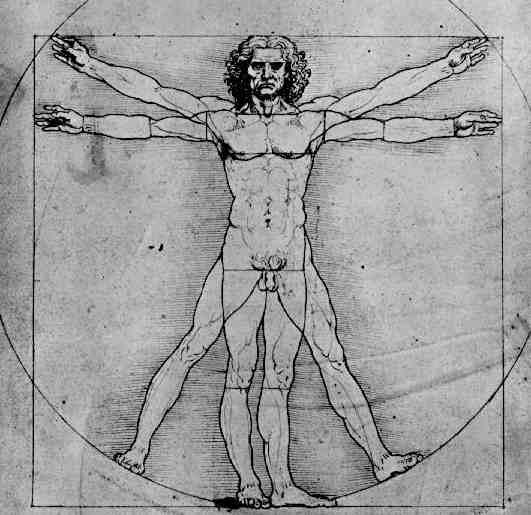
\includegraphics[height=50mm]{Figs/da-vinci-man.jpg}
\end{minipage}
\hspace{15mm}
\begin{minipage}[t]{50mm}
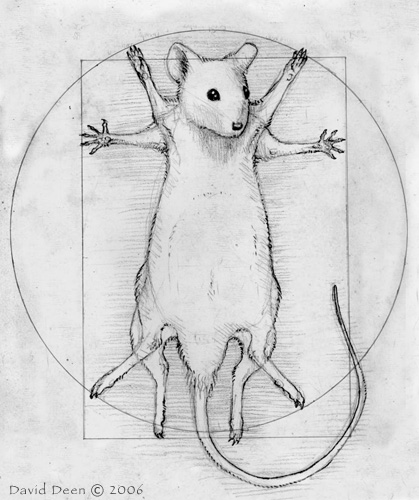
\includegraphics[height=50mm]{Figs/vitruvian_mouse.jpg}
\hspace{5mm}
\href{http://daviddeen.com}{\scriptsize \lolit \tt daviddeen.com}
\end{minipage}
}


\note{
Mice are not humans, but you can learn a great deal about human
biology and disease from mice.

The figure on the right is from David Deen.
}

\end{frame}


\begin{frame}[c]{Intercross}

\figh{Figs/intercross.pdf}{1.0}

\note{
}
\end{frame}


\begin{frame}[c]{QTL mapping}

\vspace{5mm}
\only<1 | handout 0>{\figh{Figs/lodcurve_insulin.pdf}{0.9}}
\only<2>{\figh{Figs/lodcurve_insulin_with_effects.pdf}{0.9}}

\note{
}
\end{frame}


\begin{frame}[c]{}

\figh{Figs/mouse_on_chips.png}{1.0}

\note{
I've mostly focused on a mapping genes affecting a single phenotype,
but in the past decade, I've become swamped with data.

This is a picture of a pile of gene expression arrays. More and more,
we're seeing genome-scale phenotype information. For example, in
one of my collaborations, we have data on 500 mice, each with gene
expression microarrays for 6 different tissues.

We're interested in identifying genes that control the expression of
other genes.
}

\end{frame}




\begin{frame}[c]{B6 $\times$ BTBR, \emph{Lep}$^{\text{\emph{ob}/\emph{ob}}}$}
\figw{Figs/plot-eqtl.pdf}{1.1}

\note{
    \vspace*{-12pt}
    In collaboration with Alan Attie, we've been studying
    a B6$\times$BTBR intercross, with all mice knocked out for leptin
    (and so obese), in order to understand obesity-induced diabetes.

    There are 500 intercross mice, phenotyped at a large number of
    clinical traits, and also with gene expression microarray data on
    6 tissues. These were custom two-color Agilent arrays.

    This figure shows the basic result of single-QTL genome scan for
    each expression trait, one at a time, in each tissue. Each dot is
    an inferred QTL. The y-axis is the location of the corresponding
    microarray probe, and the x-axis is the location of the QTL.

    We see a prominent diagonal, of local-eQTL, and numerous prominent
    vertical bands: ``\emph{trans}-eQTL hotspots'' where genotype at a give
    region is associated with the mRNA expression of numerous genes across
    the genome. Some of these \emph{trans}-eQTL hotspots are specific
    to a given tissue (e.g. islet chr 6) and some are seen in many
    tissues (e.g. chr 17).

    We seek to fine-map these \emph{trans}-eQTL hotspots, and to
    determine whether they involve one or multiple eQTL.
}

\end{frame}


\begin{frame}[c]{Chr 6}
\figw{Figs/chr6_lod.pdf}{1.1}

\note{
  I'm particularly interested in the locus on chromosome 6, which
  affects like 8\% of genes in pancreatic islets, but is entirely
  specific to islets.

  Each dot corresponds to the peak LOD score of a single expression
  trait: the LOD score vs the position at which it occurred. The blue
  dots are for expression traits that exist on other chromosomes; the
  brown dots are for expression traits that reside on chromosome 6.

  The local-eQTL are similar for the six tissues, but the hotspot on
  distal chr 6 in islets is seen only in islets.

  Assuming this is a single gene, how can we define a precise interval
  for the gene? We'd like to refine the localization and
  actually determine the responsible gene.
}

\end{frame}


\begin{frame}[c]{}
\centerline{\Large \ticolor Consider the non-recombinants\dots}

\note{
  Our key strategy is to focus on the non-recombinant mice (that is,
  those mice that have no recombination event in the region of this
  eQTL). For these mice, we \emph{know} their QTL genotype. We can use
  this to establish the distribution of the multivariate expression
  phenotype in each genotype group.
}

\end{frame}


\begin{frame}<handout:0>[c]{Islet c6 PCs}
\figh{Figs/islet_c6_pca_norec.pdf}{0.8}
\end{frame}

\begin{frame}[c]{Islet c6 PCs}
\addtocounter{framenumber}{-1}
\figh{Figs/islet_c6_pca.pdf}{0.8}

\note{
  We focused on the 177 microarray probes that are not on chromosome 6
  and that map to this region with LOD score $>$ 100.

  We exclude expression traits that reside on chromosome 6, thinking
  that they might be affected by separate, local-eQTL rather than the
  present locus of interest.

  We first focus on mice that had no recombination event in the 10 cM
  interval surrounding the eQTL, apply principal components analysis,
  and make a scatter plot of the first two principal components. Each
  dot is a mouse. There are three clear clusters which correspond to
  the three possible QTL genotypes.

  There were 74 mice that showed a recombination event in the
  interval; they all fall clearly into one of the three clusters.
  We can infer their eQTL genotype based on the cluster into which
  they fall.

  In this manner, the multivariate gene expression phenotype is
  converted to a co-dominant Mendelian phenotype.
}

\end{frame}


\begin{frame}<handout:0>[c]{Fine-mapping the c6 locus}
\figw{Figs/islet_c6_geno_A.pdf}{1.1}
\end{frame}

\begin{frame}<handout:0>[c]{Fine-mapping the c6 locus}
\addtocounter{framenumber}{-1}
\figw{Figs/islet_c6_geno_B.pdf}{1.1}
\end{frame}

\begin{frame}[c]{Fine-mapping the c6 locus}
\addtocounter{framenumber}{-1}
\figw{Figs/islet_c6_geno_C.pdf}{1.1}

\note{
  Using these inferred eQTL genotypes, we can locate the QTL to a
  single 3.5 Mbp interval between two markers (top panel). There are
  29 mice (highlighted) that showed a recombination event in that
  interval.

  Genotyping an additional four markers in the interval in 28/29 of
  these mice (for one mouse, DNA was not available) reduced the QTL
  interval to 900 kbp (lower-left panel). There were eight mice
  (highlighted) that showed a recombination event in this interval.

  Additional genotyping of these eight mice reduced the QTL interval
  to 298 kbp. This interval contains just three genes. Additional
  genotyping cannot exclude any of these genes.

  Our best candidate is \emph{Slco1a6}, which is a transporter of bile
  acids, some of which can have large effect on gene expression. B6
  and BTBR show a number of coding variants in this gene, one of which
  is plausibly functional. Bruno Hagenbuch at the University of Kansas
  Medical Center has shown that the two variants differ in activity,
  but we've not completely proven that \emph{Slco1a6} is responsible
  for the huge expression difference in pancreatic islets.
}

\end{frame}



\begin{frame}[c]{}
\centerline{\Large \ticolor Is it one QTL?}

\note{
  We now turn to the ``dissection'' part of the talk.

  That chromosome 6 eQTL for islets looked like a single gene, but how
  can we tell? We've developed a number of graphical diagnostics, plus
  a formal statistical test of one vs two QTL for a \emph{trans}-eQTL
  hotspot.
}

\end{frame}


\begin{frame}[c]{}
\centerline{\Large \ticolor Consider the QTL effects\dots}

\note{
  First, let's look at the effects of the QTL on the expression traits
  that map to the region.
}

\end{frame}



\begin{frame}[c]{eQTL effects: Islet c6}
\figw{Figs/effects_islet6.pdf}{1.2}

\note{
  Here's the islet c6 locus we've been studying. On the left is a plot
  of LOD score vs QTL position; we're using a signed LOD score, with
  the sign taken from the estimated additive effect of the QTL on the
  corresponding expression trait. (Each dot is a single expression
  trait.)

  On the right is a plot of the estimated dominance effect vs the
  estimated additive effect.

  The QTL looks to be additive for all expression traits, and there
  are approximately equal numbers of traits where the B6 allele is
  associated with increased and decreased expression.
}

\end{frame}

\begin{frame}[c]{eQTL effects: Kidney c13}
\figw{Figs/effects_kidney13.pdf}{1.2}

\note{
  Here's a \emph{trans}-eQTL hotspot on chr 13, for kidney. We're
  considering a pretty wide interval here, but the pattern is
  interesting and instructive.

  There looks to be a QTL at about 57 cM, and then another at about 68
  cM. For the proximal locus, the B6 allele is associated with
  decreased expression for all traits. The distal locus has the
  opposite pattern, though there are some in each direction.

  In the right panel, we see that there are a group of traits where
  the BTBR allele is dominant, and from the combination of the two
  figures, we can infer that these correspond to the proximal locus. At
  the distal locus, the B6 allele is dominant.

  That the two loci show such distinctive inheritance patterns is
  strong evidence that they are in fact distinct.

  Of course, they're rather far apart, and so we'd probably come to
  this conclusion anyway. But imagine the case that these were sitting
  just 5 cM apart. Consideration of the QTL effects could be useful.
}

\end{frame}

\begin{frame}[c]{eQTL effects: Islet c2}
\figw{Figs/effects_islet2.pdf}{1.2}

\note{
  Here's another example: islet, chr 2. This is a bit of a muddle.

  Note the additive effects, in both directions.
}

\end{frame}

\begin{frame}[c]{eQTL effects: Liver c17}
\figw{Figs/effects_liver17.pdf}{1.2}

\note{
Here's liver, chr 17. Again, not clear evidence for two QTL. Here,
BTBR looks to be dominant, but again with effects in both directions.
}

\end{frame}

\begin{frame}[c]{eQTL effects: Adipose c10}
\figw{Figs/effects_adipose10.pdf}{1.2}

\note{
One last example: adipose, chr 10. Again, no clear evidence for two
QTL, but note the two expression traits with large effects, mapping to
54 cM.

Again, BTBR looks to be dominant, and again with effects in both
directions.
}

\end{frame}



\begin{frame}[c]{}
  \centering
  \Large \ticolor
  Compare the recombinants \\
  and non-recombinants.

\note{
A second strategy is to compare the recombinants and
non-recombinants, much as we'd done in fine-mapping the islet chr 6
locus.

We can use the non-recombinants to establish the relationship between
eQTL genotype and the multivariate expression phenotype. If the
effects are strong, we should be able to discern three clear
clusters. If there's a single QTL, the recombinants should fit clearly
within these three clusters.
}

\end{frame}


\begin{frame}[c]{LDA \& PCA: Islet c6}
\figw{Figs/ldapca_islet6.pdf}{1.2}

\note{
Here's the islet chr 6 locus again.

On the left, we use linear
discriminant analysis to form a classifier of genotype based on
expression phenotype, using just the non-recombinant mice.
On the right, we use principal component analysis, again just with the
non-recombinant mice.

We look to see whether the recombinant mice fall into the clusters
defined by the non-recombinant mice.

In this case, the recombinants look just like the non-recombinants,
which is consistent with there being a single eQTL.

Note that the PCA figure (on the right) is a bit different than the
one I'd shown earlier. We're focusing on the top 50 expression traits
here; before we looked at all traits mapping with LOD $>$ 100.
}

\end{frame}

\begin{frame}[c]{LDA \& PCA: Kidney c13}
\figw{Figs/ldapca_kidney13.pdf}{1.2}

\note{
  Here's kidney chr 13.

  The three clusters are not so clearly defined. The recombinants
  don't look too different from the non-recombinants, but it's all a
  bit of a mess. These ideas aren't always helpful.
}

\end{frame}

\begin{frame}[c]{LDA \& PCA: Islet c2}
\figw{Figs/ldapca_islet2.pdf}{1.2}

\note{
  Here's islet chr 2. The LDA plot shows distinct clusters for the
  non-recombinant mice. PCA is a bit of a mess. As we'll see, the PCA
  figure is always a bit of a mess. We prefer LDA for this.

  Most interesting: the recombinant mice (in yellow) {\hilit don't}
  all fall within the clusters defined by the non-recombinant
  mice. This is good evidence for there being multiple QTL in the
  region.
}

\end{frame}

\begin{frame}[c]{LDA \& PCA: Liver c17}
\figw{Figs/ldapca_liver17.pdf}{1.2}

\note{
  Here's liver chr 17. It's not as clear as the previous example, but
  it does seem that the recombinant mice are different from the
  non-recombinant mice.
}

\end{frame}

\begin{frame}[c]{LDA \& PCA: Adipose c10}
\figw{Figs/ldapca_adipose10.pdf}{1.2}

\note{
  Here's adipose chr 10. The non-recombinant clusters are quite tight,
  and some of the recombinant mice fall outside of
  those clusters, indicating multiple QTL.
}

\end{frame}





\begin{frame}[c]{Formal test for 1 vs 2 QTL}

  \begin{itemize}
  \itemsep12pt
  \item Consider a set of traits mapping to common eQTL
  \item Multivariate QTL analysis with 1 or 2 QTL
  \item With 2-QTL model, each trait affected by one or the other QTL
    \vspace*{8pt}
    \begin{itemize}
      \itemsep8pt
      \item Order traits by estimated QTL location when considered
        separately
      \item Consider cut points of the list, assign first group to one
        QTL and second group to other.
    \end{itemize}
  \item P-value: parametric bootstrap or stratified permutation
  \end{itemize}

\note{
  As a formal test of whether a \emph{trans}-eQTL hotspot is due to
  one or multiple QTL, we use multivariate QTL analysis with one- and
  two-QTL models. In the two-QTL model, each expression trait is
  affected by one or the other QTL.

  A key technical difficulty is that the two-QTL model requires
  consideration of all possible partitions of expression traits
  between the two QTL. As an approximation, we sort the traits by
  their estimated QTL locations, when considered individually, and
  then consider only cut-points on this list: $\text{\emph{p}}-1$ partitions rather
  than $2^{\text{\emph{p}}-1}$. For each cut-point, we perform a two-dimensional scan
  for the pair of QTL locations.

  We use a parametric bootstrap (simulate data from the estimated
  single-QTL model) or a stratified permutation test (permute mice
  within strata defined by genotypes at the estimated QTL location
  under the single-QTL model).
}

\end{frame}


\begin{frame}[c]{1 vs 2 QTL: Kidney c13}
\figw{Figs/formal_kidney13.pdf}{1.2}

\note{
  I'll start with a locus with clear evidence for two QTL.

  On the left: The blue and red curves are LOD profiles for the
  location of the two QTL (for the split that gave the best fit):
  slices through the 2d LOD surface, keeping the other QTL location
  fixed. The black curve is the LOD profile for the single-QTL
  model. The dots at the bottom are the estimated QTL locations for
  the expression traits, considered individually. The triangles at the
  bottom are the estimated locations of the two QTL, under the two-QTL
  model.

  On the right: the difference between the LOD score for the two-QTL
  model for a given cut-point and that for the single-QTL model, for
  each cut point.

  There's very strong evidence for two QTL here (LOD near 40), and a
  clear inference of which expression traits are affected by the left
  and the right QTL.
}

\end{frame}

\begin{frame}[c]{1 vs 2 QTL: Islet c6}
\figw{Figs/formal_islet6.pdf}{1.2}

\note{
  Here's the islet chromosome 6 locus. The two-QTL models are never
  much better than the single-QTL better. We'd conclude that there's a
  single QTL.
}

\end{frame}

\begin{frame}[c]{1 vs 2 QTL: Islet c2}
\figw{Figs/formal_islet2.pdf}{1.2}

\note{
  Here's islet chromosome 2. Again, very strong evidence for two
  QTL. It would be interesting to split off the proximal locus and
  study the distal locus on its own: it's likely that we'll find
  evidence for three QTL in this region.
}

\end{frame}

\begin{frame}[c]{1 vs 2 QTL: Liver c17}
\figw{Figs/formal_liver17.pdf}{1.2}

\note{
Liver chromosome 7: good evidence for two QTL, but it's splitting off
just the first expression trait. We should omit this one and look for
evidence for multiple QTL among the rest. The high LOD differences for
the split at 23 suggests there would still be evidence for multiple
QTL, among those traits.
}

\end{frame}

\begin{frame}[c]{1 vs 2 QTL: Adipose c10}
\figw{Figs/formal_adipose10.pdf}{1.2}

\note{
Last one: good evidence for two QTL, but it's pulling off just a
couple of expression traits. Again, it seems we might use a more
focused interval.

There is, of course, room for improvement in this method. I think the
key issue is how to pick which set of expression traits to focus
on. The results are quite dependent on this choice. Here we've been
picking out a QTL interval in a relatively arbitray way and then
choosing the 50 traits that map to that region with the largest LOD
score.
}

\end{frame}


\begin{frame}[c]{Summary}
  \begin{itemize}
  \itemsep12pt
  \item Fine-mapping a \emph{trans}-eQTL hotspot
    \begin{itemize}
    \item Consider the non-recombinants
    \item Predict QTL genotype of recombinants \\
          $\longrightarrow$ Mendelian trait
    \item Fine-map by traditional means
    \end{itemize}
  \item Large-effect locus on chr 6
    \begin{itemize}
    \item Affects expression of $\sim$8\% of genes
    \item Effects specific to pancreatic islets
    \item Looks to be \emph{Slco1a6}
    \end{itemize}
  \item Dissecting a \emph{trans}-eQTL hotspot
    \begin{itemize}
    \item Sign of eQTL effect
    \item Degree of dominance
    \item Compare recombinants and non-recombinants
    \item Formal statistical test
    \end{itemize}
  \end{itemize}

\note{
  It's always good to include a summary slide.
}

\end{frame}


\begin{frame}{Acknowledgments}

{\small
  \begin{tabular}{llll}
    \hspace{5mm} & \hspace{5mm} & \hspace{5mm} & \\[-8pt]
    \multicolumn{4}{l}{\ticolor \normalsize Univ.\ Wisconsin{\textendash}Madison} \\
    & {\vhilit Jianan Tian}        && Brian Yandell \\
    & Alan Attie                  && Angie Oler \\
    & Mark Keller                 && Mary Rabagalia \\
    & Aimee Teo Broman            && Kathryn Schueler \\
    & Christina Kendziorski       && Donald Stapleton \\[8pt]
    \multicolumn{4}{l}{\ticolor \normalsize Univ.\ Kansas Medical Center} \\
    & Bruno Hagenbuch && Wen Zhao \\[8pt]
    \multicolumn{4}{l}{\ticolor \normalsize Merck \& Co., Inc.} \\
    & Amit Kulkarni \\[8pt]
    \multicolumn{4}{l}{\ticolor \normalsize Mt.\ Sinai} \\
    & Eric Schadt \\[8pt]
    \multicolumn{4}{l}{{\ticolor \normalsize NIH:} R01 GM074244, R01 DK066369}
\end{tabular}
}

\note{
  Lots of people were involved in this work.

  Jianan did the bulk of the method development and all of the
  software development and data analysis.

  The data come from Alan and Mark; Angie, Mary, Kathryn,
  and Donald did the work there. Aimee, Christina, and Brian are
  collaborating with me on the analysis.

  Amit worked out the annotation information for this custom
  microarray.

  The project was a collaboration with Eric Schadt, whose group did
  the microarrays and genotyping when he was at Rosetta.

  Bruno and Wei worked to validate the \emph{Slco1a6} gene.
}
\end{frame}


\begin{frame}[c]{}

\Large

\vspace*{10mm}
Slides: \href{http://bit.ly/Cornell2016}{\tt bit.ly/Cornell2016}

\vspace*{-7mm}
\hspace{90mm} \includegraphics[height=5mm]{Figs/cc-zero.png}

\vspace{2mm}

\href{http://kbroman.org}{\tt kbroman.org}

\vspace{2mm}

\href{https://github.com/kbroman}{\tt github.com/kbroman}

\vspace{2mm}

\href{https://twitter.com/kwbroman}{\tt @kwbroman}

\footnotesize
\vspace{12mm}

Tian J et al.\ (2015) Identification of the bile acid transporter \emph{Slco1a6\/} as a
candidate gene that broadly affects gene expression in mouse
pancreatic islets. \emph{Genetics\/} 201:1253--1262

\vspace{3mm}

Tian J et al.\ (2016) The dissection of expression quantitative trait
locus hotspots. \emph{Genetics\/} 202:1563--1574



\note{
  Here's where you can find me, as well as the slides for this talk.

  Also two papers on the work.
}
\end{frame}

\end{document}
